%
% latex-sample.tex
%
% This LaTeX source file provides a template for a typical research paper.
%

%
% Use the standard article template.
%
\documentclass{article}

% The geometry package allows for easy page formatting.
\usepackage{geometry}
\geometry{letterpaper}

% Load up special logo commands.
\usepackage{doc}

% Package for formatting URLs.
\usepackage{url}

% Packages and definitions for graphics files.
\usepackage{graphicx}
\usepackage{epstopdf}
\DeclareGraphicsRule{.tif}{png}{.png}{`convert #1 `dirname #1`/`basename #1 .tif`.png}

%
% Set the title, author, and date.
%
\title{Dream Interface for Headmaster}
\author{Chase Blokker}
\date{12/12/12}

%
% The document proper.
%
\begin{document}

% Add the title section.
\maketitle


\section{Concept}
\label{Concept}

My headmaster dream interface is an iPhone app that utilizes the built in accelerometer.  The app will adopt the same menu structure as the current headmaster, but will be converted into a user-friendly version for a touch screen smartphone interface.   What will make this smartphone app unique will be the button at the top of the home page titled “Navigate the Headmaster Labyrinth”.  When the user presses this button, an alternative interface to navigate through Headmaster will pop up.   This alternative interface will be a skeuomorphic adaptation of the classic game called Labyrinth.  The game is depicted in Figure 3, and the mockup iPhone interface is depicted in Figure 4.  When the user tilts the phone, the ball will roll in the desired direction, simulating a ball rolling down an inclined plane due to gravitational force.  The user will select a menu by getting the ball into the appropriately titled hole.  When the ball falls into the hole and disappears, a noise that sounds like a steel ball hitting wood will indicate to the user that they have selected that menu item. The page will then be refreshed to the selected menu item.  The user will be able to seamlessly switch back to the traditional interface at any point, meaning that when they switch interfaces, they will be brought to the parallel page in the other interface.  Any entered data that wasn’t saved will still be seen in the other interface.  This ability to switch interfaces is similar to Windows 8 and its ability to toggle between the new tiles interface and the more classic Windows desktop experience.


\section{Reason for Creating Two Interface Styles}
\label{Reason for Creating Two Interface Styles}

The original idea for this dream interface was to create a novel user interface that has never been thought of before.  The Labyrinth idea is very creative, yet it only caters to the usability metric of satisfaction.  Since Headmaster is an interface that people will use on a daily basis, it is impractical for them to have to navigate through the labyrinth every time they log onto Headmaster to update or find student information.  This would quickly become annoying, likely resulting in the user throwing their phone across the room.  Therefore, by having a secondary interface that caters to efficiency and error (where the labyrinth interface is the weakest), the user can simply bypass the labyrinth user interface option.  When the user feels compelled to be amazed at rolling a ball across the screen to select menu items, they have the option to do so.

\section{The "Classic" Interface}
\label{The "Classic" Interface}

\subsection{iOS Developer Library Guidelines}

As stated above, the classic interface will be the interface that caters to efficacy and low rate of user error.  This interface will follow several guidelines pertaining to iOS applications.  Below is a selected list found in the iOS Developer Library:\\

\begin{itemize}
\item  Controls should look tappable

The buttons should include contours and gradients, and be distinguishable from things that aren’t buttons.  In the classic interface Figures 1 and 2, these contours and gradients aren’t as distinct as they should be.  This is due to the author’s lack of Photoshop mastery.  When a button is selected, it will turn blue and stay blue, as the buttons have the ability to toggle between menu items.  The color blue is chosen due to the somewhat universal blue color choice for iOS button selection.\\

\item App structure should be clean and easy to navigate

The application will be as minimalistic as possible by choose subtle grey colors and avoiding too many options.\\

\item Design for touch

This means that you can’t simply replicate the web Headmaster interface for an iOS application.  Event driven programming for both platforms is different, as there are different events that occur.  For example, in a touch screen interface, multiple fingers can touch the screen at once and independently manipulate items.  This can’t happen with a mouse, as there is only one mouse cursor.  Likewise, with a mouse interface, the user can hover over an object, which can call an event like animation.  A user cannot hover their finger over a traditional touchscreen.  Therefore, a hover event doesn’t exist for touchscreens.\\

\item Let people scroll

According to the iOS developer library, scrolling is an easy and expected user experience.  Trying to squeeze everything within the dimensions of the phone may result in small and hard to read font size.  Therefore, scrolling both vertically and horizontally will be used in the headmaster smartphone application.\\
\end{itemize}

Now that you have a general overview of the guidelines I will try to follow, lets get into the nuts and bolts of the classic interface.  


\subsection{Login Screen}

When the app is first opened, the user will be prompted with a login screen similar to the current web-app implementation of headmaster.  This should be clean, with just two fields, username and password.  Above those two fields will be a welcome text, and below will be a login button.

\subsection{Homescreen}

The homescreen is depicted below in Figure 1.  At the top there is a menu bar for general search and logout functionality (see section 3.5 for search implementation).  This menu bar will always appear at the top of the screen, no matter what page the user is viewing, or if the user is scrolling up and down.  This will allow for higher efficiency when the user wants to logout or search, but are scrolled half way down the page.  Therefore, the user would not have to scroll back up to the top to logout or search.  Below the menu bar is a large button that says “Navigate the Headmaster Labyrinth”.  When the user presses this button, they will be directed to the alternative Labyrinth user interface.  This button only appears on the homescreen.  When navigating away from the homescreen, it will animate to the left until it is off the screen.  Similarly to how the iPhone notification menu can be swiped down from above, the Labyrinth button can be swiped from the right, and then pressed (this may interfere with swiping left and right for the student menu explained below in section 3.4.  It should also be clear to the user that they can swipe the button back so they aren’t wondering where the button went).\\

In the middle of the homescreen is a dialog that welcomes the user to Headmaster and gives them basic instructions on where to begin.\\

At the bottom on the homescreen is the menu bar for toggling between students, events, grants, and reports.  Like the search and logout menu par at the top, this menu will always exist.


\subsection{Sub-menu Example (Students)}

When the user clicks on the student button, the user will see four buttons at the top that read create, freshman, sophomore, junior, and senior.  If the user taps on one of these buttons, it will bring them to the corresponding list.  The user can then scroll up and down the screen to look through the list of students.  The search bar at top will remain at the top even when the user scrolls down.   Also, the top bar should include different ways of categorizing students (alphabetically, major, college).  This will help the user visualize students categorically.\\

The user can alternatively navigate student year by swiping left and right through their year (like you can do on the iPhone homescreen).  When the user swipes through the years, the scrollbar button menu at the top that indicates which year you are viewing should update accordingly.  This functionality is frequency seen in applications, such as the Stocks and Weather application.


\subsection{Change to Search}

Instead of having separate search options in the dropdown menus like the current headmaster, I would create a general search bar always found at the top of the screen, as depicted in Figure 1 and 2.  The user can type whatever they desire, and the matching items will drop down in a fashion akin to Google search.  Although, there should be a search filter option, where the user can select between students, events, grants, or reports.  This will help the user filter out any unwanted search results.  Also, when the user is on one of the submenu pages like students, the default search filter criterion should be students.  It is expected that the user will want to search for students when they are scrolling through the list of students.


\section{The "Labyrinth" Interface}

People know how gravity works (excluding the clumsy) as it is an everyday experience, so it is intuitive how to move the ball across the screen.  This is an affordance choice that was chosen based on its intuitive properties and user familiarity with the real world.   When the user sees the ball on the screen, notices it first move with respect to the angle of the phone, they quickly grasp the idea that they have to get the ball in the labeled menu-item hole.\\

 Although this interaction style requires waiting for the ball to reach the desired menu-item location, which significantly decreases the efficiency of the interface, it will be both visually and innately satisfying with occasional use.  As stated prior, if this interaction style was required for Headmaster, which has a “get the job done” type of functionality, then the user would become quite frustrated.  This was the justification for creating the classic interface – a streamlined version to input and change data.

\subsection{Social Aspect of Labyrinth}

In order to fully cater to the satisfaction of the labyrinth user interface, and to entice the user to play with the labyrinth interface, a point scheme will be created, where the user can enter holes that bring them to actual mazes within the headmaster interface.  Within these mazes (or quests), the user can amass points by collecting coins along the way and completing these mazes.  These “quest” holes will be far away from the functional menu item holes.   The farther a user gets from the “hub” of headmaster, the more bizarre and difficult the mazes become.\\

It would be interesting if one user could interact with another user by seeing their ball.  This would be somewhat like a massively multiplayer online (MMO) game, where each user is represented as a steel ball.  You can rack up “add-ons” and special attacks to your ball, like the ability to shoot fireballs or to roll faster.

\begin{figure}
\centering
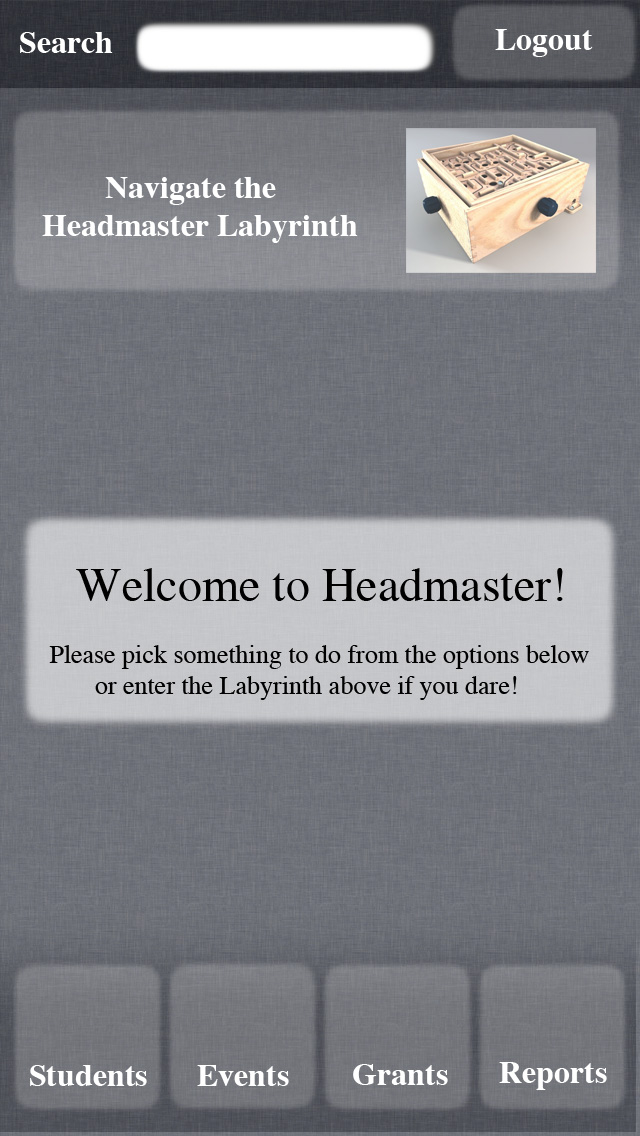
\includegraphics[width=90mm]{classic-homepage.jpg}
\caption{Example "Classic" Headmaster Interface Homescreen}
\end{figure}

\begin{figure}[ht!]
\centering
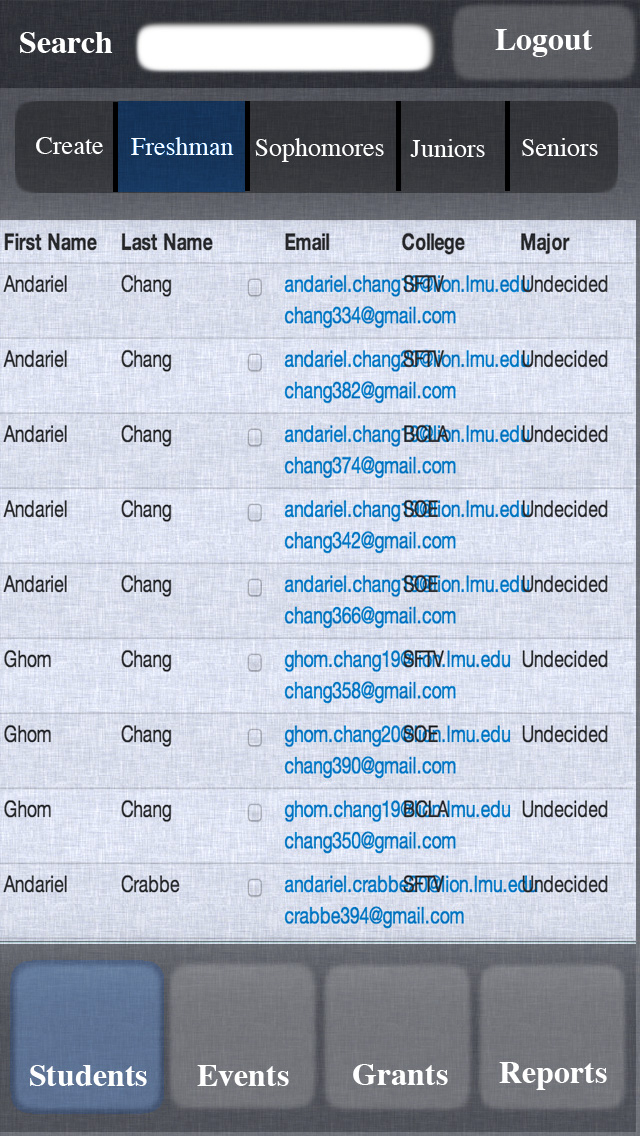
\includegraphics[width=90mm]{classic-students.jpg}
\caption{Example "Classic" Headmaster Interface Student Page}
\label{overflow}
\end{figure}

\begin{figure}[ht!]
\centering
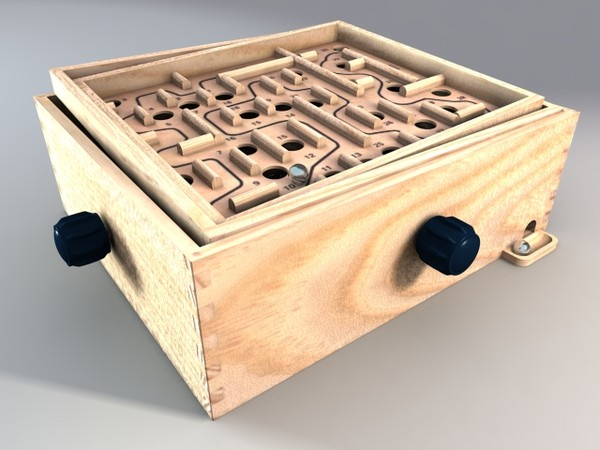
\includegraphics[width=90mm]{labyrinth.jpeg}
\caption{The game Labyrinth}
\label{overflow}
\end{figure}

\begin{figure}[ht!]
\centering
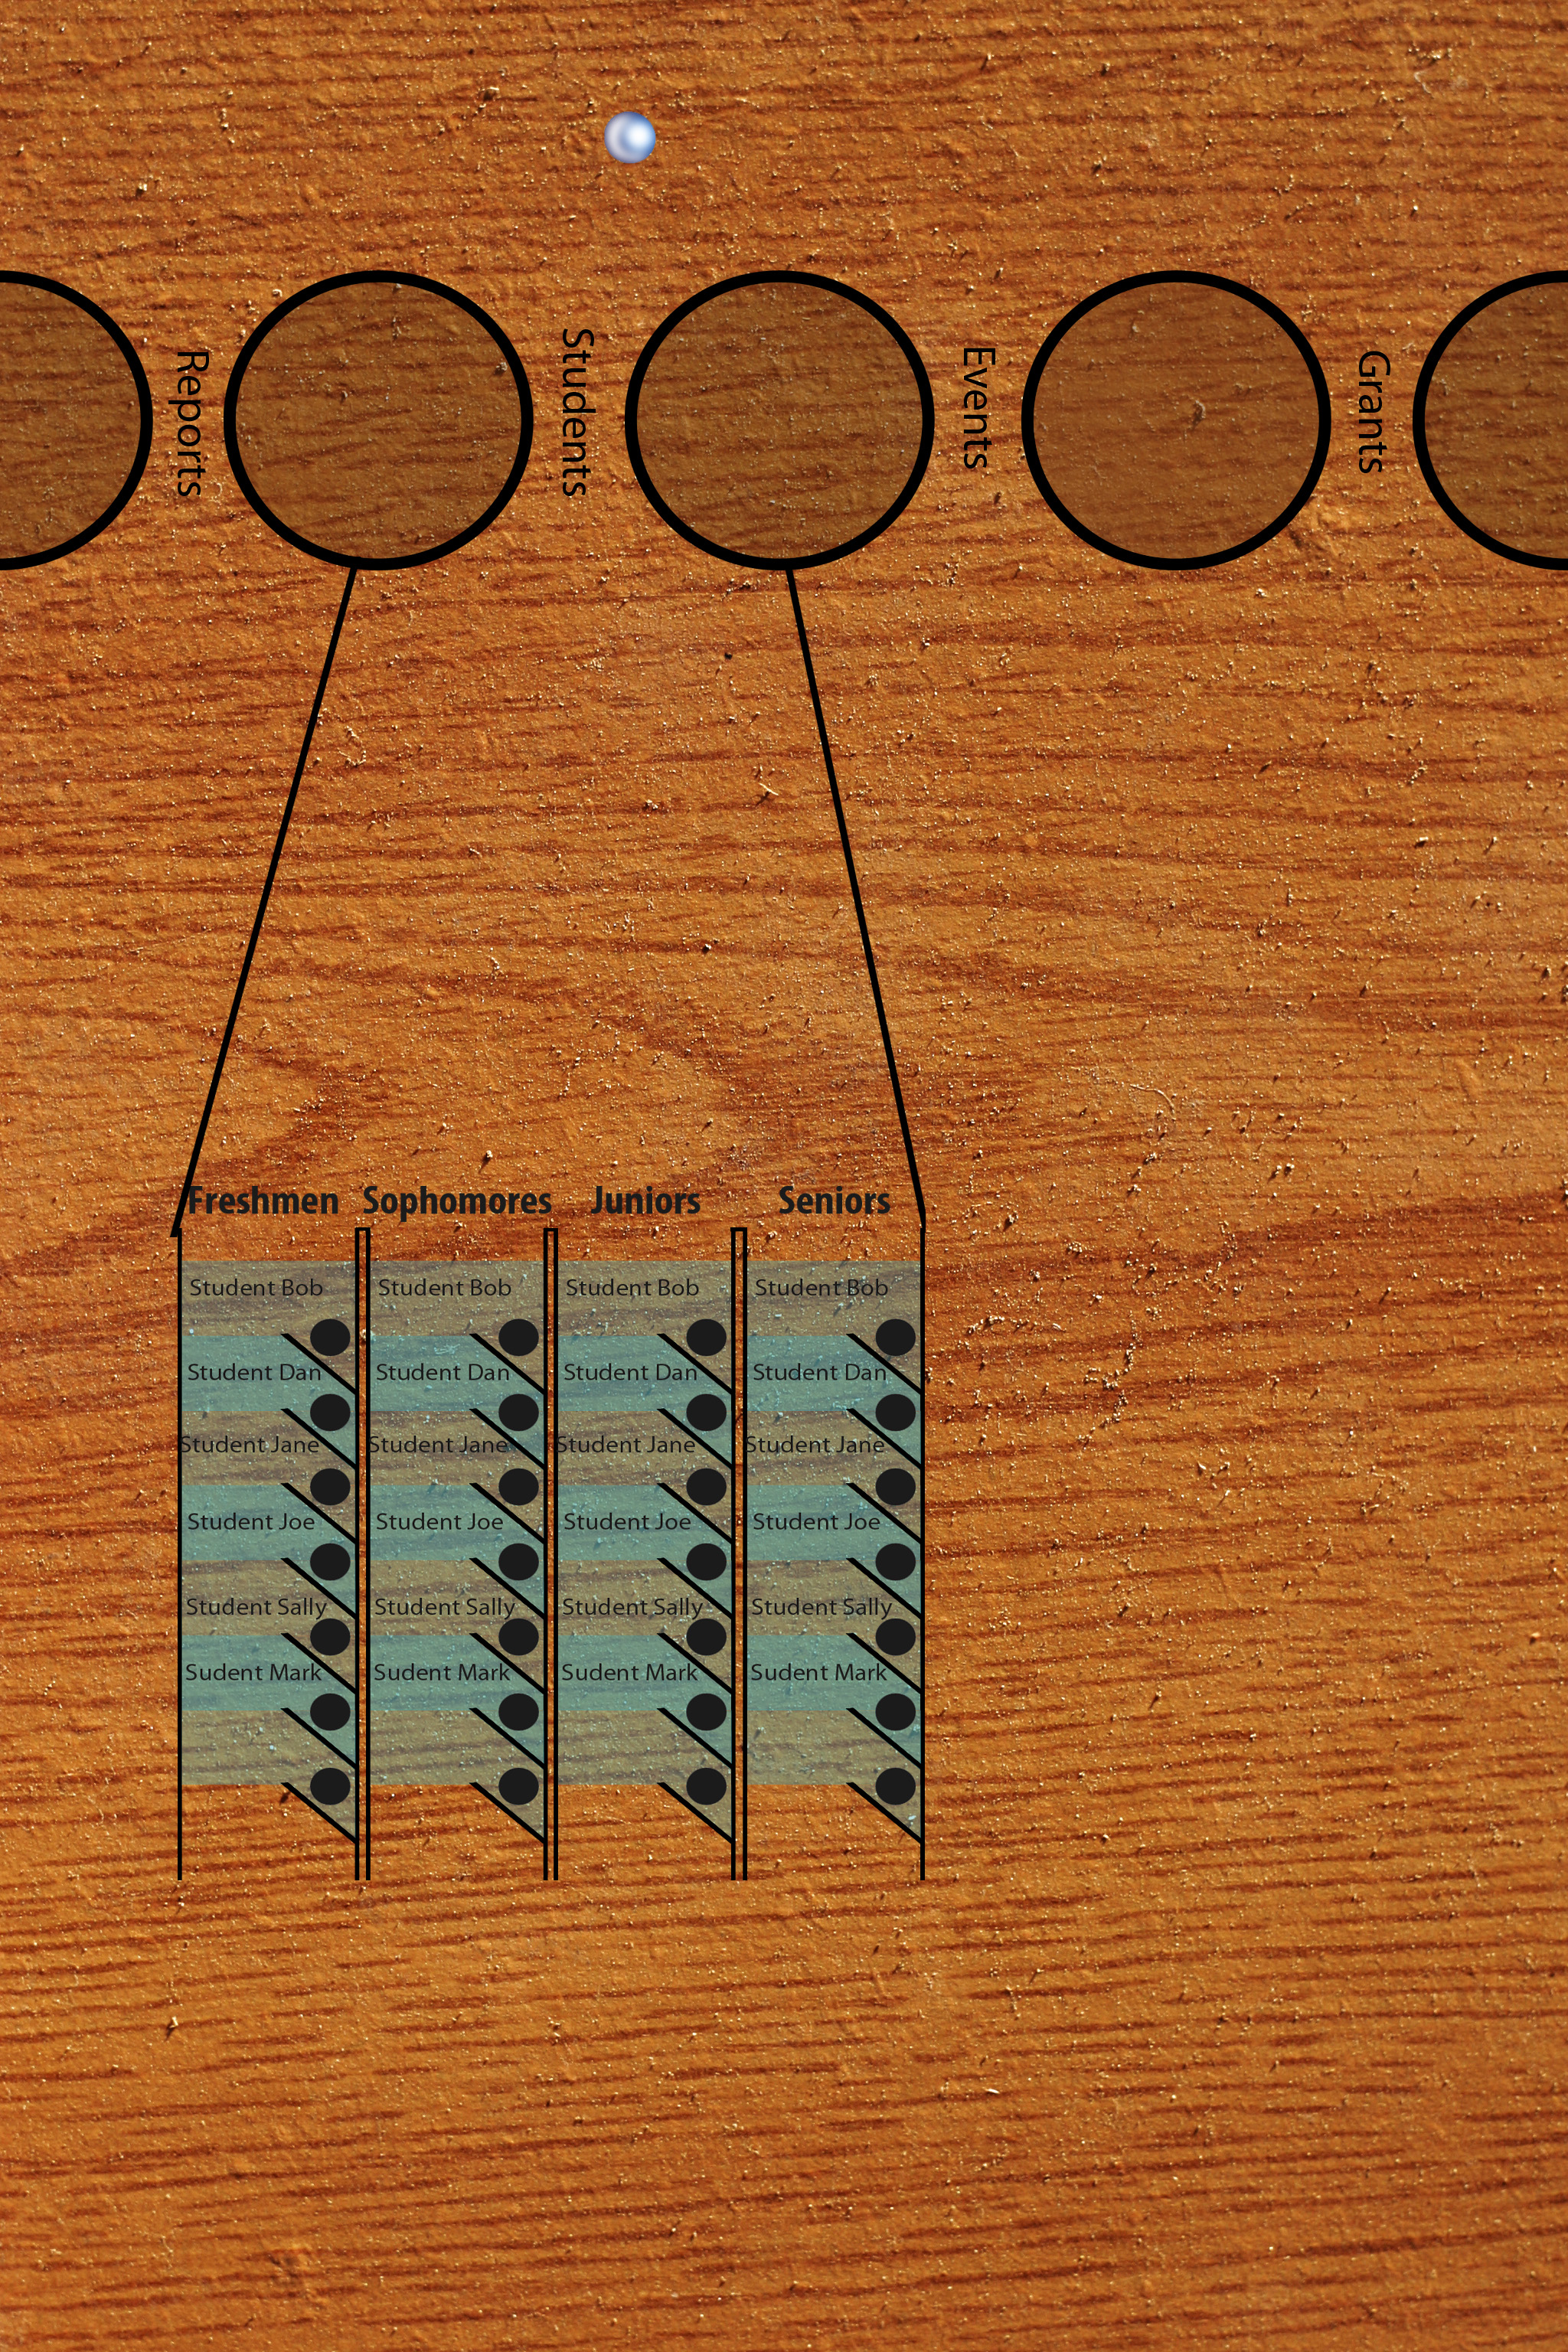
\includegraphics[width=140mm]{labyrinth-start.jpg}
\caption{Example "Labyrinth" iPhone Headmaster Interface}
\label{overflow}
\end{figure}




\end{document}